\documentclass[10pt,journal,compsoc]{IEEEtran}
\usepackage{lipsum}
\usepackage{graphicx}
\usepackage{float}
\usepackage{subfig}
\title{A Statistical Analysis of Cricket\\One Day Internationals}

\author{\textbf{Professor:} Dr. Ross Maciejewski 
\linebreak 
\linebreak
\textbf{Working Group:}
\linebreak
Aishwarya Pratap Singh (1211162781) \quad Ayushi Jain (1204841348)
\linebreak
Rahul Aakunuru (1209394573) \quad Nikhil Lohia (1211168085)}

\begin{document}

\IEEEtitleabstractindextext{
\begin{abstract}
Cricket is a game played in over a hundred countries worldwide and One Day International (ODI) is one of the most popular forms played. In this paper, we aim to find ways to effectively visualize the data generated from ODI matches. Some of the visualizations we wish to explore include stacked bar graphs, heat maps, sunburst sequence, scatter plots, and choropleth maps. Each of these visualizations is used to represent a different type of data. A combination of all the visualizations is aimed at providing a better insight to the games.
\end{abstract}

\begin{IEEEkeywords}
Cricket, performance, visualisation types
\end{IEEEkeywords}}

\maketitle

\section{Introduction}
\IEEEPARstart{C}{ricket} is an extremely popular game around the world. To put this in perspective, there were an estimated 2.2 billion viewers watching the game during the cricket world cup 2011. With cricket becoming extremely fast paced and increasingly competitive, performance analysis is steadily making its way into the team’s dressing rooms. Data visualization and data analysis in cricket has increasingly become a critical part of the game. For instance, players can try to become technically better by analyzing their own performances. Second, teams can make plans for their upcoming matches by analyzing the performance of their competitors. Third, Selectors can analyze team performance to select appropriate teams. Finally, the International Cricket Council can analyze trends to maintain the level of the games taking place. Our project aims to further investigate many such metrics that may affect the performance of a team or the popularity of the game. We present our visualizations in a way that they tell a story to the end user and let them understand how the game has progressed over the past years, in addition to how the teams have gone about looking at their performance. We try to present a visual narrative that is ``an account of a series of events, facts, etc., given in order and with the establishing of connections between them.''\cite{paper1}

\section{Related Work}
\IEEEPARstart{V}{isualizing} data in sports has always been a very popular and effective medium of displaying the performance metrics of a player or a team. There are various factors that may affect individual and team performance, such as the venue where the game is being played and tactics of the team etc \cite{paper2}. In cricket, there are a few popular methods of visualization. These methods focus on a match in general and may visualize the runs per over in an innings \cite{relatedwork1}

\begin{figure}[H]
\begin{center}
\subfloat[Bar graph representing runs per over]{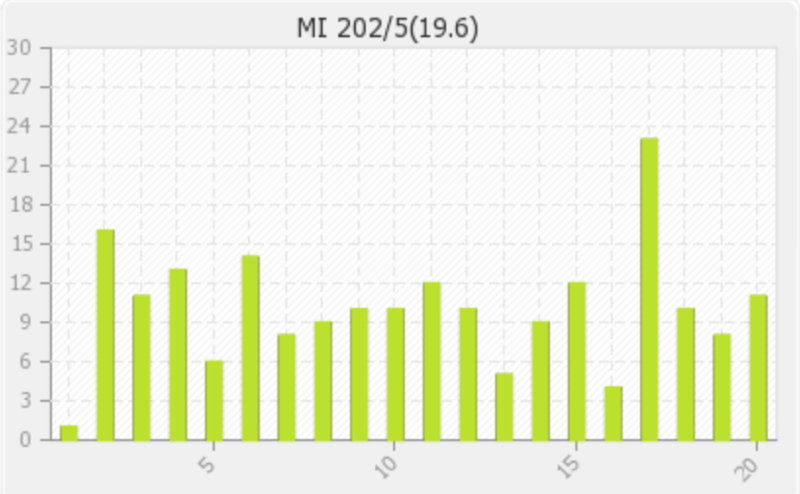
\includegraphics[width = 3in]{relatedwork1.png}}
\end{center}
\end{figure}

Another popular visualization that can be used is the line chart. Here, we are comparing the performance of the two teams competing over by over\cite{relatedwork2}

\begin{figure}[H]
\begin{center}
\subfloat[Line chart representing runs per over]{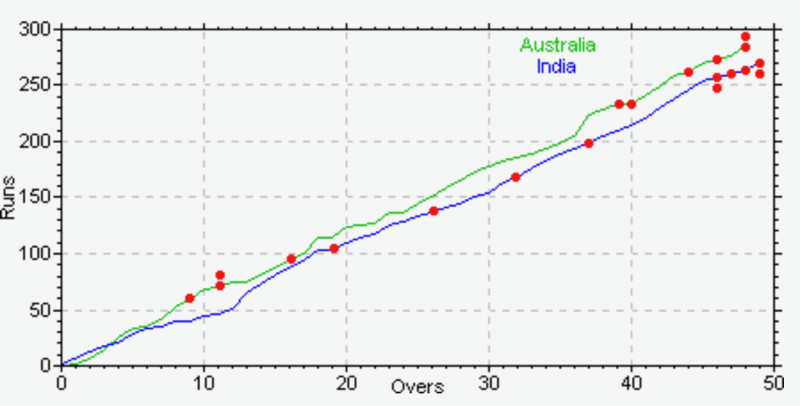
\includegraphics[width = 3in]{relatedwork2.png}}
\end{center}
\end{figure}

A visualization called a wagon-wheel can be used to depict the areas of the field where the runs were scored in\cite{relatedwork2}

\begin{figure}[H]
\begin{center}
\subfloat[Wagon wheel]{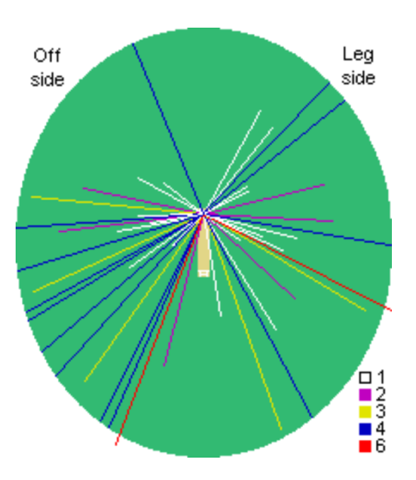
\includegraphics[width = 2.8in]{relatedwork3.png}}
\end{center}
\end{figure}

For this project, we have divided the queries into two categories: individual/team-based performance analysis and game-based performance analysis. We tried exploring the different types of visualizations that could effectively communicate these statistics to the end user.
\linebreak
\linebreak
For a visualization that represents the batsmen friendliness of a venue, we classify the various cricket venues based on the average runs being scored in the matches being played there. This presents a very interesting problem of binning the dataset. We not only need to decide what the starting point is but also on what, the division of the dataset will be. According to Gennady Andrienko, Natalia Andrienko, and Alexandr Savinov\cite{relatedwork3} there are 3 widely used methods of data classification
\begin{itemize}
\item Classification into equal intervals
\item Classification with equal frequencies of objects in the classes
\item Statistically optimal classification
\end{itemize}

\begin{figure}[H]
\begin{center}
\subfloat[Different types of classifications]{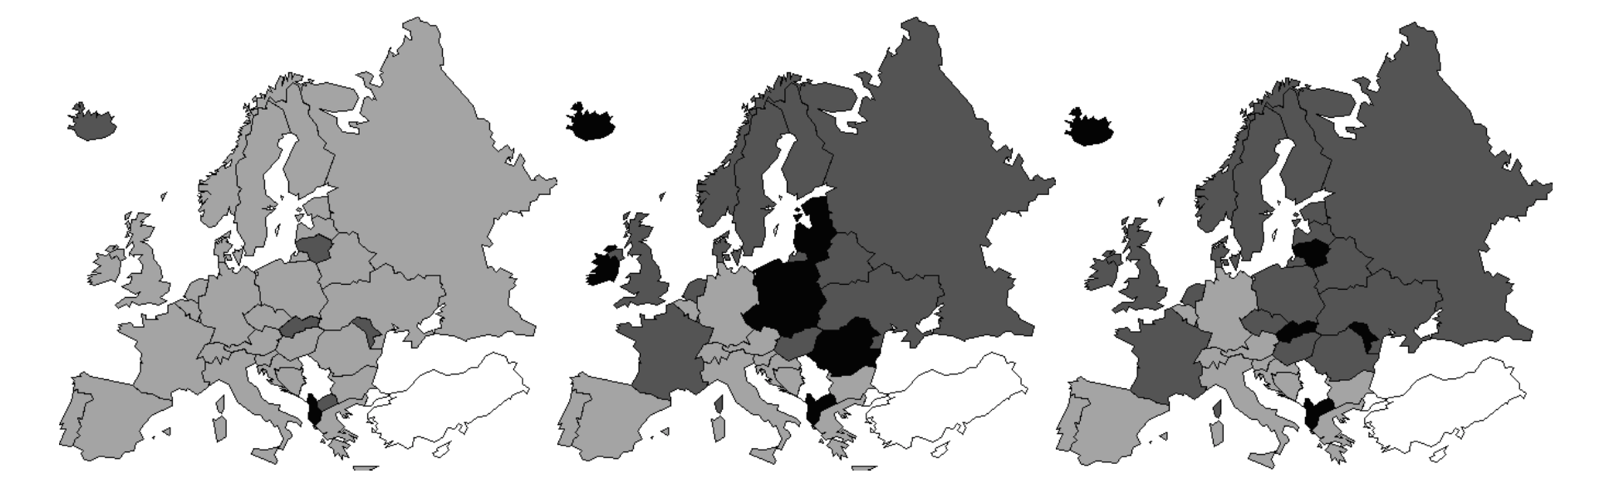
\includegraphics[width = 3.4in]{relatedwork4.png}}
\end{center}
\end{figure}

The figure above \cite{relatedwork3} shows clearly how these different types of classifications can lead to the visualization telling a completely different story. In case of cricket scores, the average scores in the various venues lie in a relatively small range between early 200s to early 300s. It would not make sense to start at 0 and divide the dataset equally in this case. Classification based on equal frequencies may also not give the true picture as two venues relatively very close in terms of average scores may lie in different bins.
\linebreak
\linebreak
The Manhattan or the bar graph is another popular visualization being used in the cricket analysis all the time along with a line chart as described earlier. \cite{relatedwork4} We are also using these graphs to show various statistics like average runs being scored by a team or analyzing the team performance over various over intervals in a game. These help in analyzing and even understanding the trends of how the team has been performing. These can be used to predict how a team is going to perform in the upcoming matches whereas can also be used by the opposition to figure out what the strong points of a team are.\cite{relatedwork4} A line graph also helps compare the performance of more than a team in the same timeline based on over intervals and hence can be used to deduce why a team does not perform as good as some other team and which time interval should they improve upon.

\begin{figure}[H]
\begin{center}
\subfloat[Wagon wheel, manhattan and worm graph]{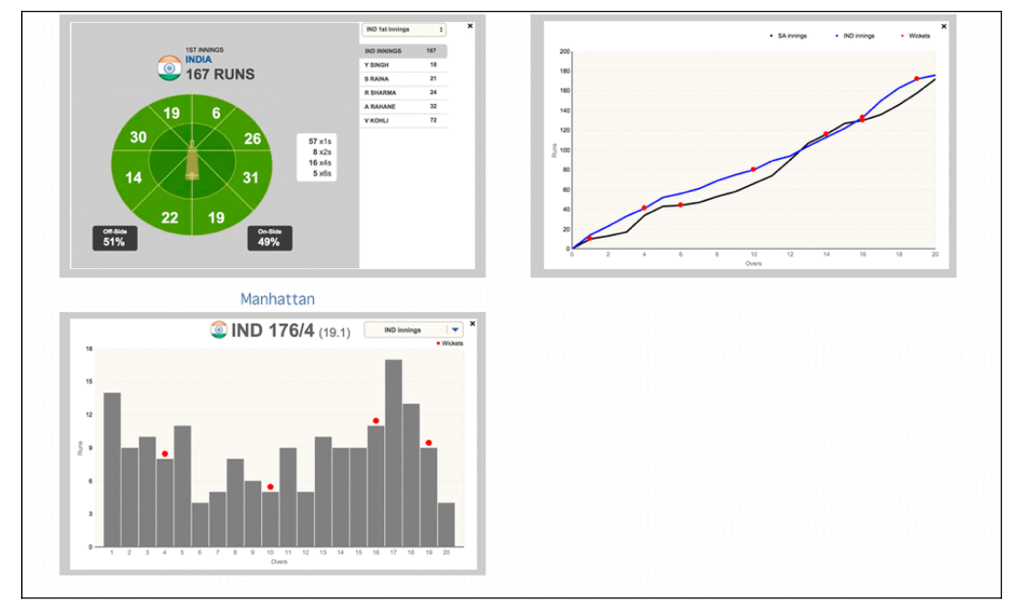
\includegraphics[width = 3.4in]{relatedwork5.png}}
\end{center}
\end{figure}

An important point of analysis is where we try to figure out if there is a relationship between a venue and team’s performance. One alternative that we thought of representing this information was by using a heat map. A heat map in a soccer game is used to represent the positions that a player frequently plays at during the game.\cite{relatedwork5} This is basically a density estimation methodology. 

\begin{figure}[H]
\begin{center}
\subfloat[Heat Map]{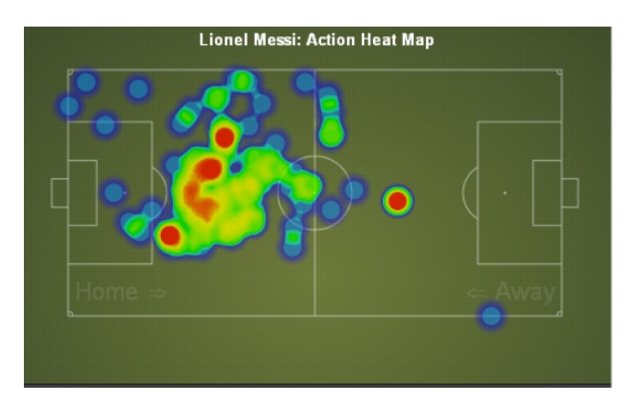
\includegraphics[width = 3.2in]{relatedwork6.png}}
\end{center}
\end{figure}

We saw a parallel in cricket and thought of representing the density of the number of wins of a country in various venues on a map as a heat map. This approach though looked perfect at first but then later we realized a big flaw in this representation. This only represents the number of wins in a venue but does not give any information regarding how many matches a team played at that venue and hence this cannot be considered a good metric to represent the information of how good a venue is for a team. Thus, an effective visualization for such a data would be a use of stacked bar graph. This clearly represents the important information to the user. It clearly shows the number of matches played by a team at a venue along with the number of matches the team won and lost at the venue. This visualization would thus be effective in finding if a team plays better at a venue and later to go and predict if there is a home advantage in the game of cricket

\section{Work done so far}
We found an interesting data set of ODI matches from 2006 to 2016 with ball by ball updates. Each match consists as a single YAML file and we have a total of 1306 matches\cite{dataset}. This gives us roughly 6 million balls to analyse. From the dataset we plan to answer the following questions
\begin{itemize}
\item Which country has maximum number of runs?
\item A team's performance in different over intervals.
\item Which venue sees the highest score?
\item What is the percentage of runs scored in boundaries by a team?
\item Which overs have more boundaries?
\end{itemize}
These questions can be derived from the statistics of a game but various other insightful questions can also be inferred. 
\begin{itemize}
\item How many times did the winning team win the toss as well?
\item How many runs must a team score to win 90\% of the matches?
\item Is there a thing as home advantage?
\end{itemize}
We plan to determine if some of the myths in a cricket game are true or not?
\begin{itemize}
\item Does a lot of boundaries result in winning a match?
\item Do extra runs really matter in determining the fate of a match?
\end{itemize}
To gain an insight into all these questions we plan to extract the following fields from our dataset
\begin{verbatim}
Date, Team1, Team2, Venue, Toss, Winner, 
Over(ex. 3.2), Runs, Extras
\end{verbatim}
We plan to visualise each of the question using a visualisation technique which is capable of giving a clear idea of the result. This visualisation would be helpful for story telling during a cricket game and predicting the result.

\section{Conclusion}
As a further part of our study we plan to parse all the data files to a CSV format and visualise all the required information. The information would be presented in form of a single scrollable webpage which would be interactive and the design elements would be tightly integrated. We also plan to explore different options for visualising certain sets of data such that it is intuitive enough at the first glance. As we continue to work, we expect to find even more co-relations and pattern between the data which could affect the outcome of a game.

\begin{thebibliography}{1}

\bibitem{paper1}
Segel E., Heer J. ``Narrative visualization: telling stories with data''. \emph{IEEE Transactions on Visualization and Computer Graphics}, 2010

\bibitem{latexcompanion}
M.~Goossens, F.~Mittelbach, A.~Samarin. \emph{The \LaTeX\ Companion},
Addison-Wesley (1994), ISBN~0-201-54199-8.

\bibitem{relatedwork1}
http://www.cricwaves.com/cricket/2662/chennai-super-kings-vs-mumbai-indians-final-t20-24-May-2015/Teammanrate.html

\bibitem{relatedwork2}
http://www.dangermouse.net/cricket/statistics.html

\bibitem{relatedwork3}
Adrienko G., Adrienko N. and Savinov A. ``Choropleth maps: Classification Revisited''. \emph{Proceedings of the 19th International Cartographic Conference}. Beijing, China. Aug. pp.1209–1219. ICA

\bibitem{relatedwork4}
Prasant Nair, ``Editing the worm graph alias ball by ball data and predicting the winner for cricket,'' \emph{International Journal of Physical Education, Sports and Health}, 2016

\bibitem{relatedwork5}
C.~Perin, R.~Vuillemot, J.~D.~Fekete, ``et al. Soccerstories: A kick-off for visual soccer analysis''. \emph{IEEE transactions on visualization and computer graphics}, 2013

\bibitem{paper2}
G.~Pingali, A.~Opalach, Y.~Jean, and I.~Carlbom,``Visualization of sports using motion trajectories: Providing insights into performance, style, and strategy,'' in \emph{Proc. IEEE Visualization, vol. 4}, 2001

\bibitem{dataset}
http://cricsheet.org/downloads/odis.zip


\end{thebibliography}

\end{document}